\section{Introduction \& Motivating Example}
\td{Since we do not mention metamorphic DSLs in title/abstract anymore, mention them here}
One of the first steps in designing a new DSL is to choose the \emph{language vehicle} within which it will be engineered.
We define a language vehicle (LV) as the technological means for implementing a language.
%A language vehicle may pertain to any \emph{technological space} (TS) such as grammarware, modelware, PLware, \etc.
The distinction between language vehicles is orthogonal to the distinction between \emph{technological spaces} (\eg~grammarware, modelware, PLware);\footnote{In this paper, we build upon \citeauthor{kurtev2002technological}'s view of a TS:~``a working context with a set of associated concepts, body of knowledge, tools, required skills, and possibilities''~\cite{kurtev2002technological}.} the distinction between graphical and textual syntaxes; the distinction between internal, embedded, and external DSLs, \etc.
%In addition, we consider a cohesive set of tools in a given TS (\eg~a particular language workbench) as a separate TS.
For instance, following this definition, we consider Rascal and Spoofax as two distinct language vehicles within the broader technological space of grammarware and meta-programming, and EMF and UML as two distinct language vehicles within the broader technological space of modelware.
LVs usually come with their own meta-languages for expressing the various aspects of a DSL:~abstract syntax, concrete syntax, static and execution semantics, tools, \etc.
Examples of prominent LV include meta-modeling environments such as EMF~\cite{steinberg2008emf}, meta-programming environments such as Rascal~\cite{klint2010easy} and Spoofax~\cite{kats2010spoofax}, projectional environments such as MPS~\cite{voelter2013language}, plain old programming languages such as Racket~\cite{felleisen2018programmable} or Scala~\cite{hofer2010modular}, and language workbenches (LWBs) in general~\cite{erdweg2015evaluating}.
\td{Sentence above could be shortened/removed}
As implementation techniques radically differ from one LV to the other, this initial design choice commits the development of a DSL in a set direction that can hardly be reconsidered later on.

From a language designer's point of view, however, every LV has its own strengths.
The ecosystem around EMF excels in the definition of, for instance, graphical editors and persistence frameworks for large models, while the Rascal environment excels in the definition of, for instance, interpreters and refactoring tools \td{need refs?}.
%On the other hand, the flexibility of manipulating the concepts of a DSL through a fluent API, using the capabilities of a general-purpose programming language, is unmatched.
The benefits of various LV are also visible from the language users' point of view.
While domain experts may prefer to manipulate domain concepts through a dedicated syntax, advanced users (\eg~system integrators) may favor the flexibility of a fluent API in their favorite programming language to manipulate the very same abstractions.
However, it is currently not possible to \emph{combine the strengths of multiple LV to engineer a single DSL}.
\td{Why?}

Let us consider a simple finite-state machine (FSM) language as a motivating example.
As depicted in \Cref{fig:motivating-fsm}, one would like to combine the strengths of multiple LVs to engineer this DSL.
Rascal could be used to develop its interpreter, a set of refactoring tools (\eg~state collapsing and minimization), and a textual editor; EMF to develop a graphical editor and animator of running FSM models; Java to offer a fluent API for advanced users who focus on its integration with other DSLs or within a broader system.

Using today's techniques, it is possible to define the same FSM language with the aforementioned tools in these three LV.
There is currently no way, however, to apply the tools of a given LV on the models created in another LV---for instance, animating a FSM model written in EMF using the Rascal interpreter, or synchronizing a textual FSM model in Rascal with its equivalent incarnation in the form of a Java AST.
Achieving this goal requires to synchronize the diverse in-memory representations of the same model in different LV; for instance to allow the Rascal interpreter to update its in-memory representation of an FSM model and synchronize it with the in-memory representation of the same model in EMF.

In this paper, we envision a language engineering activity where language designers combine tools from multiple vehicles to engineer a single DSL.
We endeavor to show \emph{how to break down the barriers between different vehicles so that language designers can benefit from the strengths of each in the engineering of a single DSL, and language users can synchronize their models across various shapes}.
%\emph{Metamorphic synchronization} refers to the possibility of synchronizing different incarnations of the same model in different shapes of a language, \ie~in different vehicles.
As different vehicles rely on radically different theories, a successful approach for bridging them must thus \emph{align} \td{!no!} them in some way.
We investigate this question in the next section.

\begin{figure}[bt]
	\centering
	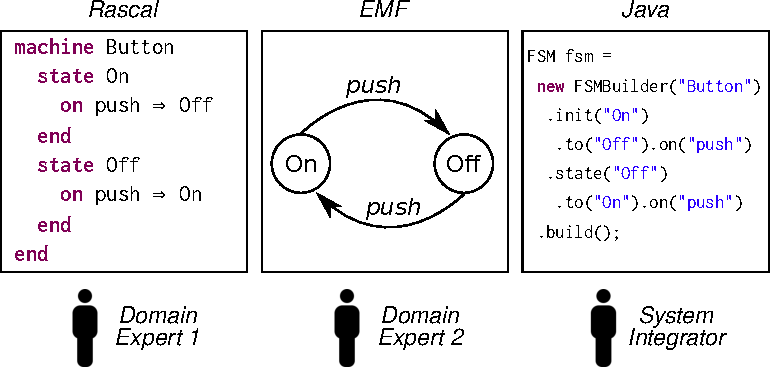
\includegraphics[width=\columnwidth]{figures/motivating-fsm-simplified}
	\caption{Three incarnations of the same FSM model:~different representations and tools for different users and tasks}
	\label{fig:motivating-fsm}
\end{figure}
